\documentclass{article}\usepackage[]{graphicx}\usepackage[]{color}
%% maxwidth is the original width if it is less than linewidth
%% otherwise use linewidth (to make sure the graphics do not exceed the margin)
\makeatletter
\def\maxwidth{ %
  \ifdim\Gin@nat@width>\linewidth
    \linewidth
  \else
    \Gin@nat@width
  \fi
}
\makeatother

\definecolor{fgcolor}{rgb}{0.345, 0.345, 0.345}
\newcommand{\hlnum}[1]{\textcolor[rgb]{0.686,0.059,0.569}{#1}}%
\newcommand{\hlstr}[1]{\textcolor[rgb]{0.192,0.494,0.8}{#1}}%
\newcommand{\hlcom}[1]{\textcolor[rgb]{0.678,0.584,0.686}{\textit{#1}}}%
\newcommand{\hlopt}[1]{\textcolor[rgb]{0,0,0}{#1}}%
\newcommand{\hlstd}[1]{\textcolor[rgb]{0.345,0.345,0.345}{#1}}%
\newcommand{\hlkwa}[1]{\textcolor[rgb]{0.161,0.373,0.58}{\textbf{#1}}}%
\newcommand{\hlkwb}[1]{\textcolor[rgb]{0.69,0.353,0.396}{#1}}%
\newcommand{\hlkwc}[1]{\textcolor[rgb]{0.333,0.667,0.333}{#1}}%
\newcommand{\hlkwd}[1]{\textcolor[rgb]{0.737,0.353,0.396}{\textbf{#1}}}%
\let\hlipl\hlkwb

\usepackage{framed}
\makeatletter
\newenvironment{kframe}{%
 \def\at@end@of@kframe{}%
 \ifinner\ifhmode%
  \def\at@end@of@kframe{\end{minipage}}%
  \begin{minipage}{\columnwidth}%
 \fi\fi%
 \def\FrameCommand##1{\hskip\@totalleftmargin \hskip-\fboxsep
 \colorbox{shadecolor}{##1}\hskip-\fboxsep
     % There is no \\@totalrightmargin, so:
     \hskip-\linewidth \hskip-\@totalleftmargin \hskip\columnwidth}%
 \MakeFramed {\advance\hsize-\width
   \@totalleftmargin\z@ \linewidth\hsize
   \@setminipage}}%
 {\par\unskip\endMakeFramed%
 \at@end@of@kframe}
\makeatother

\definecolor{shadecolor}{rgb}{.97, .97, .97}
\definecolor{messagecolor}{rgb}{0, 0, 0}
\definecolor{warningcolor}{rgb}{1, 0, 1}
\definecolor{errorcolor}{rgb}{1, 0, 0}
\newenvironment{knitrout}{}{} % an empty environment to be redefined in TeX

\usepackage{alltt}

% \usepackage[utf8]{inputenc}
\usepackage{amsmath}
\usepackage{fancyhdr}
\usepackage{array}
\usepackage{longtable}
\usepackage{graphicx}
\usepackage{color}
\usepackage[letterpaper, margin=1in]{geometry}
\usepackage{lscape}
\newcommand{\blandscape}{\begin{landscape}}
\newcommand{\elandscape}{\end{landscape}}
\usepackage{dcolumn}
\usepackage{bbm}
\usepackage{threeparttable}
\usepackage{booktabs}
\usepackage{expex}
\usepackage{pdflscape}
\usepackage{rotating, graphicx}
\usepackage{tabulary}
\usepackage{lscape}
\usepackage{makecell}
\usepackage{algorithm}
\usepackage{multirow}
\usepackage{colortbl}
\usepackage{longtable}
\usepackage{array}
\usepackage{multirow}
\usepackage{wrapfig}
\usepackage{float}
\usepackage{pdflscape}
\usepackage{tabu}
\usepackage{threeparttable}

\title{%
Homework 7\\
\large Applied Mutlivariate Analysis}
\date{October 22, 2018}
\author{Emorie Beck}
\IfFileExists{upquote.sty}{\usepackage{upquote}}{}
\begin{document}
\maketitle
% \SweaveOpts{concordance=TRUE}

\section{Workspace}
\subsection{Packages}



\begin{knitrout}
\definecolor{shadecolor}{rgb}{0.969, 0.969, 0.969}\color{fgcolor}\begin{kframe}
\begin{alltt}
\hlkwd{library}\hlstd{(car)}
\hlkwd{library}\hlstd{(knitr)}
\hlkwd{library}\hlstd{(psych)}
\hlkwd{library}\hlstd{(kableExtra)}
\hlkwd{library}\hlstd{(MASS)}
\hlkwd{library}\hlstd{(vegan)}
\hlkwd{library}\hlstd{(smacof)}
\hlkwd{library}\hlstd{(scatterplot3d)}
\hlkwd{library}\hlstd{(ape)}
\hlkwd{library}\hlstd{(ade4)}
\hlkwd{library}\hlstd{(ecodist)}
\hlkwd{library}\hlstd{(lme4)}
\hlkwd{library}\hlstd{(plyr)}
\hlkwd{library}\hlstd{(tidyverse)}
\end{alltt}
\end{kframe}
\end{knitrout}



\subsection{data}
We know that President Trump is a polarizing figure within the United States, but how is he viewed around the world? In 2017, the Pew Research Center conducted surveys in 38 countries. Each sample was representative of that country’s adult population and sample sizes were typically around 1000 in each country (the details can be found at http://www.pewresearch.org/methodology/international-survey-research/international- methodology/global-attitudes-survey/all-country/2017). Included among the survey items were the following that asked respondents to answer “yes” or “no”:  

\textit{Please tell me whether you think the following describes U.S. President Donald Trump. Do you think of Donald Trump as \_\_\_\_\_\_\_\_\_\_?} 
\begin{enumerate}
\item well-qualified to be president
\item a strong leader
\item dangerous
\item charismatic
\item intolerant
\item caring about ordinary people
\item arrogant
\end{enumerate}
The data are contained in the file, trump.csv. For each country, the percentage of the sample that responded “yes” is provided.

\begin{knitrout}
\definecolor{shadecolor}{rgb}{0.969, 0.969, 0.969}\color{fgcolor}\begin{kframe}
\begin{alltt}
\hlstd{wd} \hlkwb{<-} \hlstr{"https://github.com/emoriebeck/homeworks/raw/master/multivariate/homeworks/homework7"}

\hlstd{dat} \hlkwb{<-} \hlkwd{sprintf}\hlstd{(}\hlstr{"%s/trump.csv"}\hlstd{, wd)} \hlopt
  \hlkwd{read.csv}\hlstd{(.,} \hlkwc{stringsAsFactors} \hlstd{= F)}

\hlkwd{head}\hlstd{(dat)}
\end{alltt}
\begin{verbatim}
##          Country well_qualified strong_leader intolerant dangerous
## 1 United States              38            52         60        53
## 2        Canada              16            38         78        72
## 3        France              21            54         83        78
## 4       Germany               6            44         81        76
## 5        Greece              33            55         70        55
## 6       Hungary              39            60         50        42
##   charismatic caring_ordinary arrogant
## 1          49              42       81
## 2          37              23       93
## 3          52              18       93
## 4          37              13       91
## 5          35              20       78
## 6          58              33       66
\end{verbatim}
\end{kframe}
\end{knitrout}

\section{Question 1}
First, provide a profile of the sample. Construct a bar graph that contains the mean percentage for each question along with the 95\% confidence interval.  

\begin{knitrout}
\definecolor{shadecolor}{rgb}{0.969, 0.969, 0.969}\color{fgcolor}\begin{kframe}
\begin{alltt}
\hlstd{dat} \hlopt
  \hlkwd{gather}\hlstd{(}\hlkwc{key} \hlstd{= item,} \hlkwc{value} \hlstd{= value,} \hlopt{-}\hlstd{Country)} \hlopt
  \hlstd{Rmisc}\hlopt{::}\hlkwd{summarySE}\hlstd{(.,} \hlkwc{measurevar} \hlstd{=} \hlstr{"value"}\hlstd{,} \hlkwc{groupvars} \hlstd{=} \hlstr{"item"}\hlstd{)} \hlopt
  \hlkwd{mutate}\hlstd{(}\hlkwc{rank} \hlstd{=} \hlkwd{rank}\hlstd{(}\hlkwd{desc}\hlstd{(value)))} \hlopt
  \hlkwd{arrange}\hlstd{(rank)} \hlopt
  \hlkwd{mutate}\hlstd{(}\hlkwc{item} \hlstd{=} \hlkwd{factor}\hlstd{(item,} \hlkwc{levels} \hlstd{=} \hlkwd{unique}\hlstd{(item)))} \hlopt
  \hlkwd{ggplot}\hlstd{(}\hlkwd{aes}\hlstd{(}\hlkwc{x} \hlstd{= item,} \hlkwc{y} \hlstd{= value,} \hlkwc{ymin} \hlstd{= value} \hlopt{-} \hlstd{ci,} \hlkwc{ymax} \hlstd{= value} \hlopt{+} \hlstd{ci))} \hlopt{+}
    \hlkwd{geom_bar}\hlstd{(}\hlkwd{aes}\hlstd{(}\hlkwc{fill} \hlstd{= item),} \hlkwc{color} \hlstd{=} \hlstr{"black"}\hlstd{,} \hlkwc{position} \hlstd{=} \hlstr{"dodge"}\hlstd{,} \hlkwc{stat} \hlstd{=} \hlstr{"identity"}\hlstd{)} \hlopt{+}
    \hlkwd{geom_errorbar}\hlstd{(}\hlkwc{position} \hlstd{=} \hlstr{"dodge"}\hlstd{,} \hlkwc{width} \hlstd{=} \hlnum{.1}\hlstd{)} \hlopt{+}
    \hlkwd{labs}\hlstd{(}\hlkwc{y} \hlstd{=} \hlstr{"Mean Percentage"}\hlstd{,} \hlkwc{x} \hlstd{=} \hlkwa{NULL}\hlstd{)} \hlopt{+}
    \hlkwd{coord_flip}\hlstd{()} \hlopt{+}
    \hlkwd{theme_classic}\hlstd{()} \hlopt{+}
    \hlkwd{theme}\hlstd{(}\hlkwc{legend.position} \hlstd{=} \hlstr{"none"}\hlstd{)}
\end{alltt}
\end{kframe}
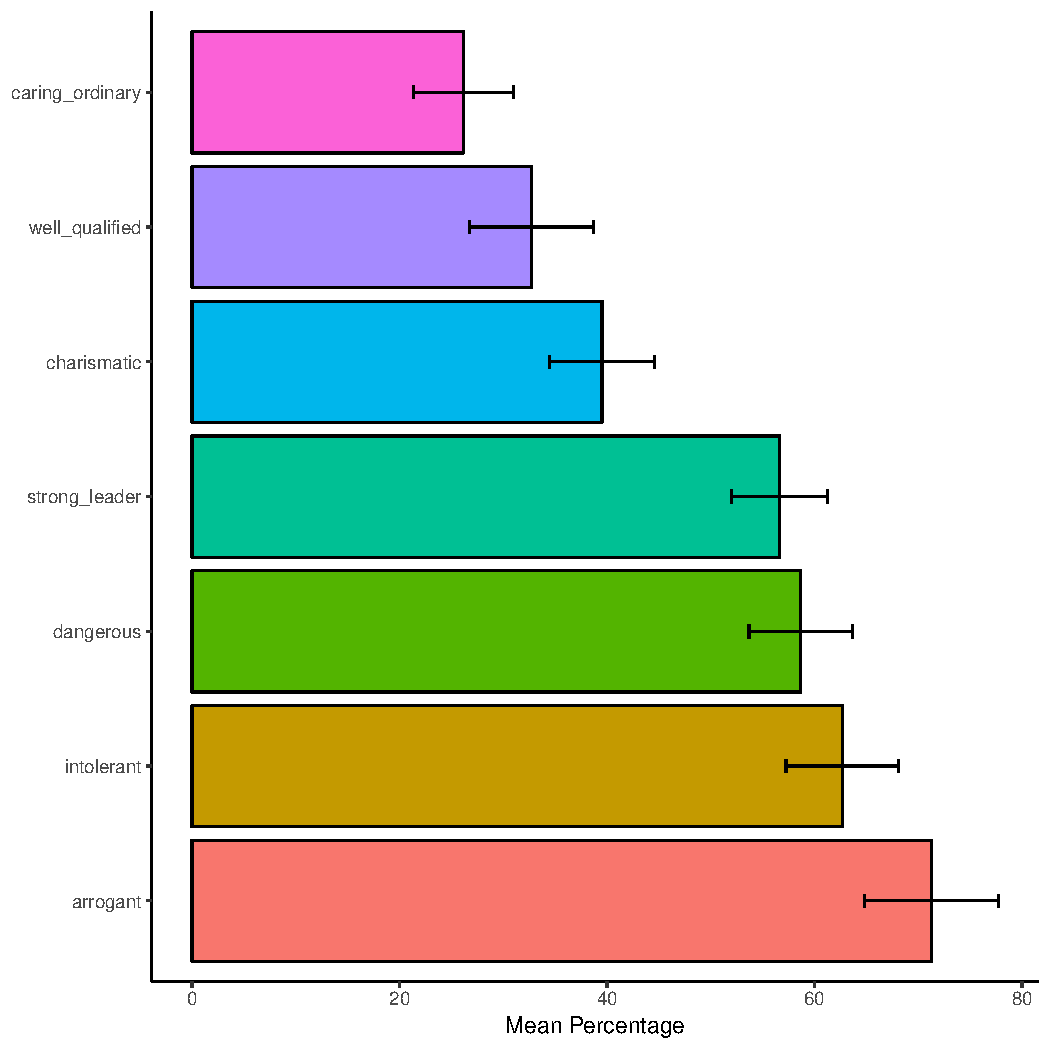
\includegraphics[width=\maxwidth]{figure/unnamed-chunk-4-1} 

\end{knitrout}

\section{Question 2}
Second, create two additional data frames representing alternative ways to represent the data.

\begin{knitrout}
\definecolor{shadecolor}{rgb}{0.969, 0.969, 0.969}\color{fgcolor}\begin{kframe}
\begin{alltt}
\hlstd{GGally}\hlopt{::}\hlkwd{ggpairs}\hlstd{(dat} \hlopt \hlkwd{select}\hlstd{(}\hlopt{-}\hlstd{Country))}
\end{alltt}
\end{kframe}
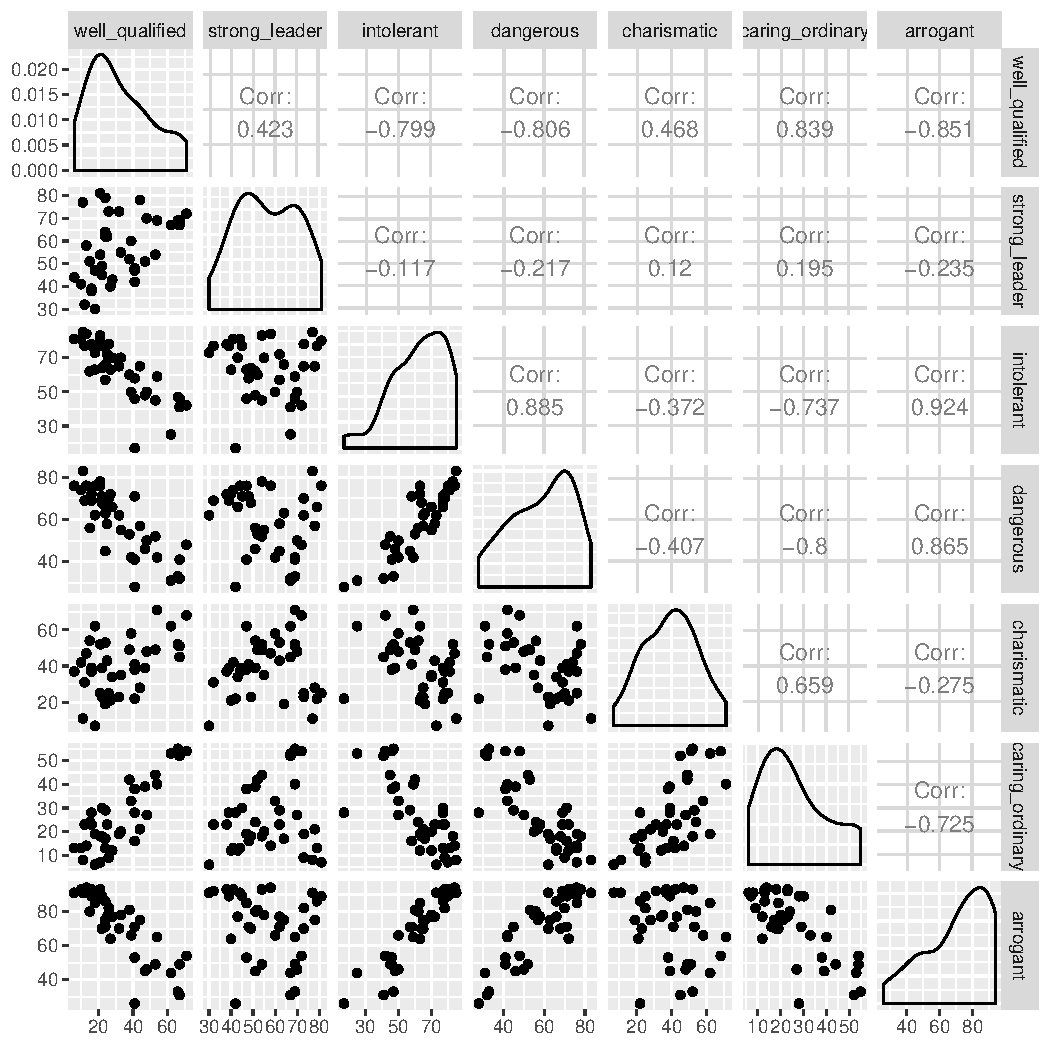
\includegraphics[width=\maxwidth]{figure/unnamed-chunk-5-1} 
\begin{kframe}\begin{alltt}
\hlstd{dat} \hlopt \hlkwd{gather}\hlstd{(}\hlkwc{key} \hlstd{= item,} \hlkwc{value} \hlstd{= value,} \hlopt{-}\hlstd{Country)} \hlopt
  \hlkwd{group_by}\hlstd{(item)} \hlopt
  \hlkwd{mutate}\hlstd{(}\hlkwc{mean} \hlstd{=} \hlkwd{mean}\hlstd{(value))} \hlopt
  \hlkwd{ungroup}\hlstd{()} \hlopt
  \hlkwd{mutate}\hlstd{(}\hlkwc{rank} \hlstd{=} \hlkwd{rank}\hlstd{(}\hlkwd{desc}\hlstd{(mean)))} \hlopt
  \hlkwd{arrange}\hlstd{(rank)} \hlopt
  \hlkwd{mutate}\hlstd{(}\hlkwc{item} \hlstd{=} \hlkwd{factor}\hlstd{(item,} \hlkwc{levels} \hlstd{=} \hlkwd{unique}\hlstd{(item)))}  \hlopt
  \hlkwd{ggplot}\hlstd{(}\hlkwd{aes}\hlstd{(}\hlkwc{x} \hlstd{= value,} \hlkwc{y} \hlstd{= item,} \hlkwc{fill} \hlstd{= item))} \hlopt{+}
    \hlcom{# geom_boxplot() + }
    \hlstd{ggridges}\hlopt{::}\hlkwd{geom_density_ridges}\hlstd{()} \hlopt{+}
    \hlkwd{labs}\hlstd{(}\hlkwc{x} \hlstd{=} \hlstr{"Percentage"}\hlstd{,} \hlkwc{y} \hlstd{=} \hlkwa{NULL}\hlstd{,} \hlkwc{title} \hlstd{=} \hlstr{"Density Distributions"}\hlstd{)} \hlopt{+}
    \hlkwd{theme_classic}\hlstd{()} \hlopt{+}
    \hlkwd{theme}\hlstd{(}\hlkwc{legend.position} \hlstd{=} \hlstr{"none"}\hlstd{,}
          \hlkwc{plot.title} \hlstd{=} \hlkwd{element_text}\hlstd{(}\hlkwc{hjust} \hlstd{=} \hlnum{.5}\hlstd{,} \hlkwc{face} \hlstd{=} \hlstr{"bold"}\hlstd{))}
\end{alltt}
\end{kframe}
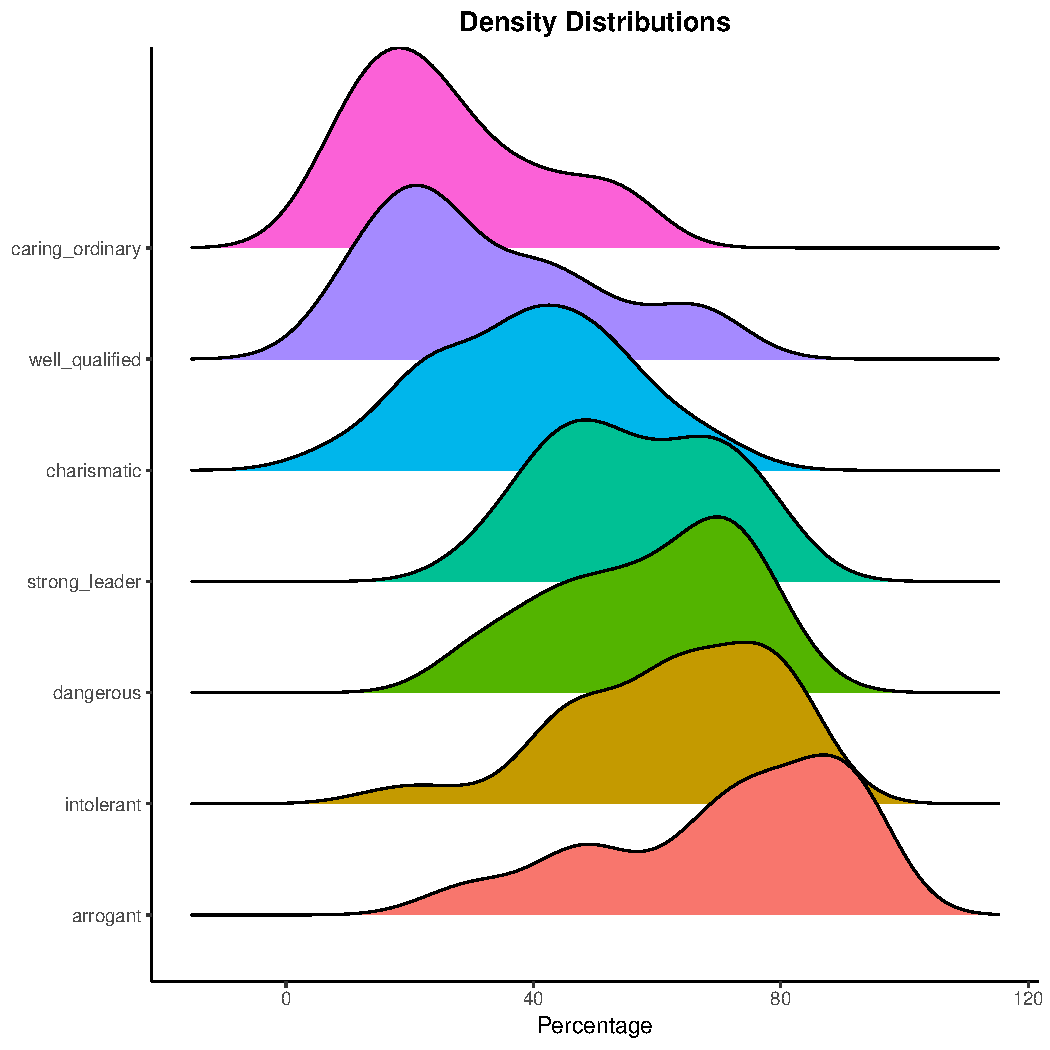
\includegraphics[width=\maxwidth]{figure/unnamed-chunk-5-2} 

\end{knitrout}


\subsection{Part A}
The ratings are in a common metric (percentages) but vary in their standard deviations. To give each item equal weight, standardize the ratings.

\begin{knitrout}
\definecolor{shadecolor}{rgb}{0.969, 0.969, 0.969}\color{fgcolor}\begin{kframe}
\begin{alltt}
\hlstd{dat} \hlkwb{<-} \hlstd{dat} \hlopt
  \hlkwd{gather}\hlstd{(}\hlkwc{key} \hlstd{= item,} \hlkwc{value} \hlstd{= raw,} \hlopt{-}\hlstd{Country)} \hlopt
  \hlkwd{group_by}\hlstd{(item)} \hlopt
  \hlkwd{mutate}\hlstd{(}\hlkwc{z} \hlstd{=} \hlkwd{as.numeric}\hlstd{(}\hlkwd{scale}\hlstd{(raw)))}
\end{alltt}
\end{kframe}
\end{knitrout}


\subsection{Part B}
The percentage scale is bounded and a case might be made that differences at the extremes (e.g., the difference between 90\% and 95\%) are more important than equal differences in the middle (e.g., the difference between 45\% and 50\%). One way to provide this unequal emphasis is to convert the percentages to proportions and then to transform them to probits using the qnorm( ) function. This will stretch the scale at the extremes.

\begin{knitrout}
\definecolor{shadecolor}{rgb}{0.969, 0.969, 0.969}\color{fgcolor}\begin{kframe}
\begin{alltt}
\hlstd{dat} \hlkwb{<-} \hlstd{dat} \hlopt
  \hlkwd{mutate}\hlstd{(}\hlkwc{probit} \hlstd{= ecotoxicology}\hlopt{::}\hlkwd{PercentageToProbit}\hlstd{(raw}\hlopt{/}\hlnum{100}\hlstd{))}
\end{alltt}
\end{kframe}
\end{knitrout}


\section{Question 3}
Convert each rating file to a distance matrix using Euclidean distances.  

\begin{knitrout}
\definecolor{shadecolor}{rgb}{0.969, 0.969, 0.969}\color{fgcolor}\begin{kframe}
\begin{alltt}
\hlstd{nested.dat} \hlkwb{<-} \hlstd{dat} \hlopt
  \hlkwd{gather}\hlstd{(}\hlkwc{key} \hlstd{= type,} \hlkwc{value} \hlstd{= value,} \hlopt{-}\hlstd{Country,} \hlopt{-}\hlstd{item)} \hlopt
  \hlkwd{spread}\hlstd{(}\hlkwc{key} \hlstd{= item,} \hlkwc{value} \hlstd{= value)} \hlopt
  \hlkwd{group_by}\hlstd{(type)} \hlopt
  \hlkwd{nest}\hlstd{()} \hlopt
  \hlkwd{mutate}\hlstd{(}\hlkwc{d_mat} \hlstd{=} \hlkwd{map}\hlstd{(data,} \hlopt{~}\hlkwd{dist}\hlstd{(.[,}\hlopt{-}\hlnum{1}\hlstd{],}\hlkwc{method}\hlstd{=}\hlstr{"euclidean"}\hlstd{,}\hlkwc{diag}\hlstd{=}\hlnum{TRUE}\hlstd{)))}
\end{alltt}
\end{kframe}
\end{knitrout}


\section{Question 4}
Using the original ratings data, and metric multidimensional scaling, construct a plot of the stress values (for up to 6 dimensions). How many dimensions are suggested by this plot?

\begin{knitrout}
\definecolor{shadecolor}{rgb}{0.969, 0.969, 0.969}\color{fgcolor}\begin{kframe}
\begin{alltt}
\hlstd{nested.dat} \hlkwb{<-} \hlstd{nested.dat} \hlopt
  \hlkwd{full_join}\hlstd{(}\hlkwd{crossing}\hlstd{(}\hlkwc{type} \hlstd{= nested.dat}\hlopt{$}\hlstd{type,} \hlkwc{dim} \hlstd{=} \hlnum{1}\hlopt{:}\hlnum{6}\hlstd{))} \hlopt
  \hlkwd{mutate}\hlstd{(}\hlkwc{mds} \hlstd{=} \hlkwd{map2}\hlstd{(d_mat, dim,} \hlopt{~}\hlkwd{smacofSym}\hlstd{(.x,} \hlkwc{ndim} \hlstd{= .y,}\hlkwc{verbose}\hlstd{=}\hlnum{FALSE}\hlstd{,}\hlkwc{type}\hlstd{=}\hlstr{"ordinal"}\hlstd{,}\hlkwc{itmax}\hlstd{=}\hlnum{1000}\hlstd{)),}
         \hlkwc{stress} \hlstd{=} \hlkwd{map_dbl}\hlstd{(mds,} \hlopt{~}\hlstd{.}\hlopt{$}\hlstd{stress))}

\hlstd{nested.dat} \hlopt
  \hlkwd{filter}\hlstd{(type} \hlopt{==} \hlstr{"raw"}\hlstd{)} \hlopt
  \hlkwd{ggplot}\hlstd{(}\hlkwd{aes}\hlstd{(}\hlkwc{x} \hlstd{= dim,} \hlkwc{y} \hlstd{= stress))} \hlopt{+}
    \hlkwd{geom_line}\hlstd{()} \hlopt{+}
    \hlkwd{geom_point}\hlstd{()} \hlopt{+}
    \hlkwd{scale_x_continuous}\hlstd{(}\hlkwc{limits} \hlstd{=} \hlkwd{c}\hlstd{(}\hlnum{1}\hlstd{,}\hlnum{6}\hlstd{),} \hlkwc{breaks} \hlstd{=} \hlnum{1}\hlopt{:}\hlnum{6}\hlstd{)} \hlopt{+}
    \hlkwd{labs}\hlstd{(}\hlkwc{x} \hlstd{=} \hlstr{"Number of Dimensions"}\hlstd{,} \hlkwc{y} \hlstd{=} \hlstr{"Stress"}\hlstd{,} \hlkwc{title} \hlstd{=} \hlstr{"Question 4: Stress Plot"}\hlstd{)} \hlopt{+}
    \hlkwd{theme_classic}\hlstd{()} \hlopt{+}
    \hlkwd{theme}\hlstd{(}\hlkwc{plot.title} \hlstd{=} \hlkwd{element_text}\hlstd{(}\hlkwc{face} \hlstd{=} \hlstr{"bold"}\hlstd{,} \hlkwc{hjust} \hlstd{=} \hlnum{.5}\hlstd{),}
          \hlkwc{axis.text} \hlstd{=} \hlkwd{element_text}\hlstd{(}\hlkwc{face} \hlstd{=} \hlstr{"bold"}\hlstd{,} \hlkwc{color} \hlstd{=} \hlstr{"black"}\hlstd{),}
          \hlkwc{axis.title} \hlstd{=} \hlkwd{element_text}\hlstd{(}\hlkwc{face} \hlstd{=} \hlstr{"bold"}\hlstd{))}
\end{alltt}
\end{kframe}
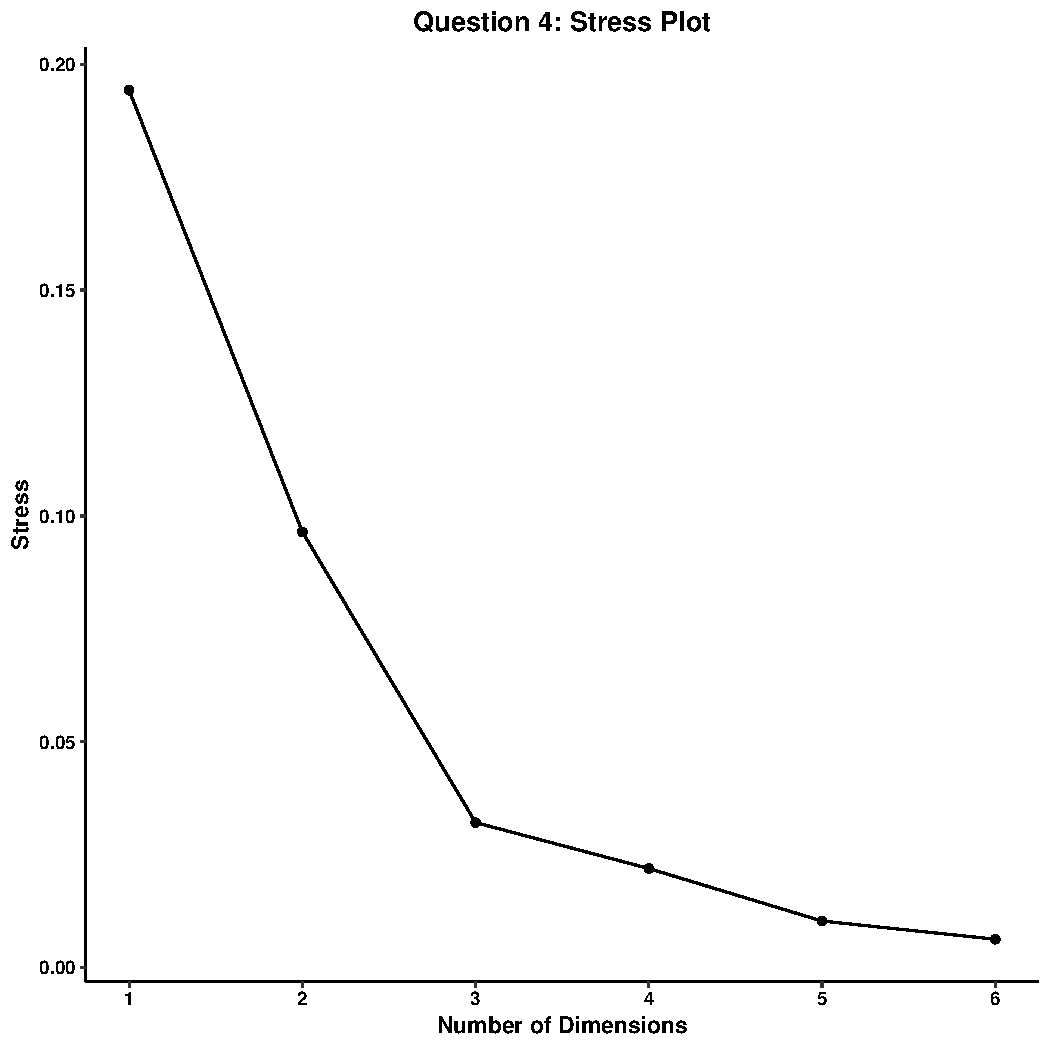
\includegraphics[width=\maxwidth]{figure/unnamed-chunk-9-1} 

\end{knitrout}

There appear to be 3 dimensions.

\section{Question 5}
Construct Shepard plots for up to 4 dimensions. Is your decision about the number of dimensions in Question 4 supported by the Shepard plots?  

\begin{knitrout}
\definecolor{shadecolor}{rgb}{0.969, 0.969, 0.969}\color{fgcolor}\begin{kframe}
\begin{alltt}
\hlstd{shep_extract_fun} \hlkwb{<-} \hlkwa{function}\hlstd{(}\hlkwc{shep}\hlstd{)\{}
  \hlkwd{tibble}\hlstd{(}\hlkwc{Dissimilarity} \hlstd{= shep}\hlopt{$}\hlstd{x,} \hlkwc{Distance} \hlstd{= shep}\hlopt{$}\hlstd{yf)}
\hlstd{\}}

\hlstd{nested.dat} \hlkwb{<-} \hlstd{nested.dat} \hlopt
  \hlkwd{mutate}\hlstd{(}\hlkwc{shep} \hlstd{=} \hlkwd{map2}\hlstd{(d_mat, mds,} \hlopt{~}\hlkwd{Shepard}\hlstd{(.x,.y}\hlopt{$}\hlstd{conf)),}
         \hlkwc{shep_val} \hlstd{=} \hlkwd{map}\hlstd{(shep, shep_extract_fun))}

\hlstd{nested.dat} \hlopt
  \hlkwd{unnest}\hlstd{(shep_val)} \hlopt
  \hlkwd{filter}\hlstd{(dim} \hlopt{<=} \hlnum{4} \hlopt{&} \hlstd{type} \hlopt{==} \hlstr{"raw"}\hlstd{)} \hlopt
  \hlkwd{ggplot}\hlstd{(}\hlkwd{aes}\hlstd{(}\hlkwc{x} \hlstd{= Dissimilarity,} \hlkwc{y} \hlstd{= Distance,} \hlkwc{color} \hlstd{=} \hlkwd{factor}\hlstd{(dim)))} \hlopt{+}
    \hlkwd{geom_point}\hlstd{()} \hlopt{+}
    \hlkwd{facet_wrap}\hlstd{(}\hlopt{~}\hlstd{dim)} \hlopt{+}
    \hlkwd{theme_classic}\hlstd{()} \hlopt{+}
    \hlkwd{theme}\hlstd{(}\hlkwc{legend.position} \hlstd{=} \hlstr{"none"}\hlstd{)}
\end{alltt}
\end{kframe}
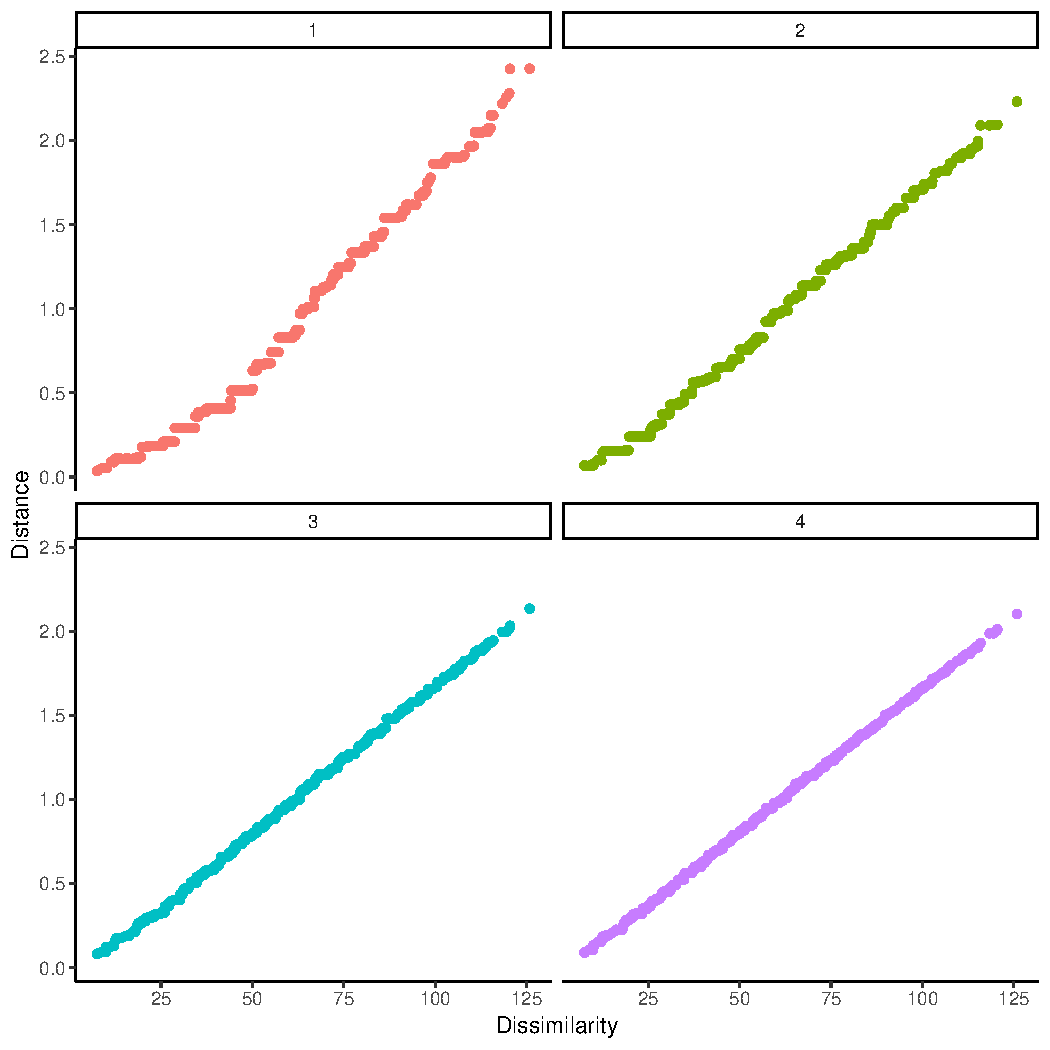
\includegraphics[width=\maxwidth]{figure/unnamed-chunk-10-1} 

\end{knitrout}

The Shepard plot also suggests 3 dimensions.

\section{Question 6}
Construct a graphical display of the multidimensional space using the number of dimensions identified in Question 4.

\begin{knitrout}
\definecolor{shadecolor}{rgb}{0.969, 0.969, 0.969}\color{fgcolor}\begin{kframe}
\begin{alltt}
\hlstd{mds_3_dat} \hlkwb{<-} \hlstd{(nested.dat} \hlopt
  \hlkwd{filter}\hlstd{(dim} \hlopt{==} \hlnum{3} \hlopt{&} \hlstd{type} \hlopt{==} \hlstr{"raw"}\hlstd{))}\hlopt{$}\hlstd{mds[[}\hlnum{1}\hlstd{]]}\hlopt{$}\hlstd{conf} \hlopt
  \hlstd{data.frame}

\hlkwd{scatterplot3d}\hlstd{(}\hlkwc{x} \hlstd{= mds_3_dat}\hlopt{$}\hlstd{D1,} \hlkwc{y} \hlstd{= mds_3_dat}\hlopt{$}\hlstd{D2,} \hlkwc{z} \hlstd{= mds_3_dat}\hlopt{$}\hlstd{D3,}
              \hlkwc{xlab} \hlstd{=} \hlstr{"Dimension 1"}\hlstd{,} \hlkwc{ylab} \hlstd{=} \hlstr{"Dimension 2"}\hlstd{,} \hlkwc{zlab} \hlstd{=} \hlstr{"Dimension 3x"}\hlstd{)}
\end{alltt}
\end{kframe}
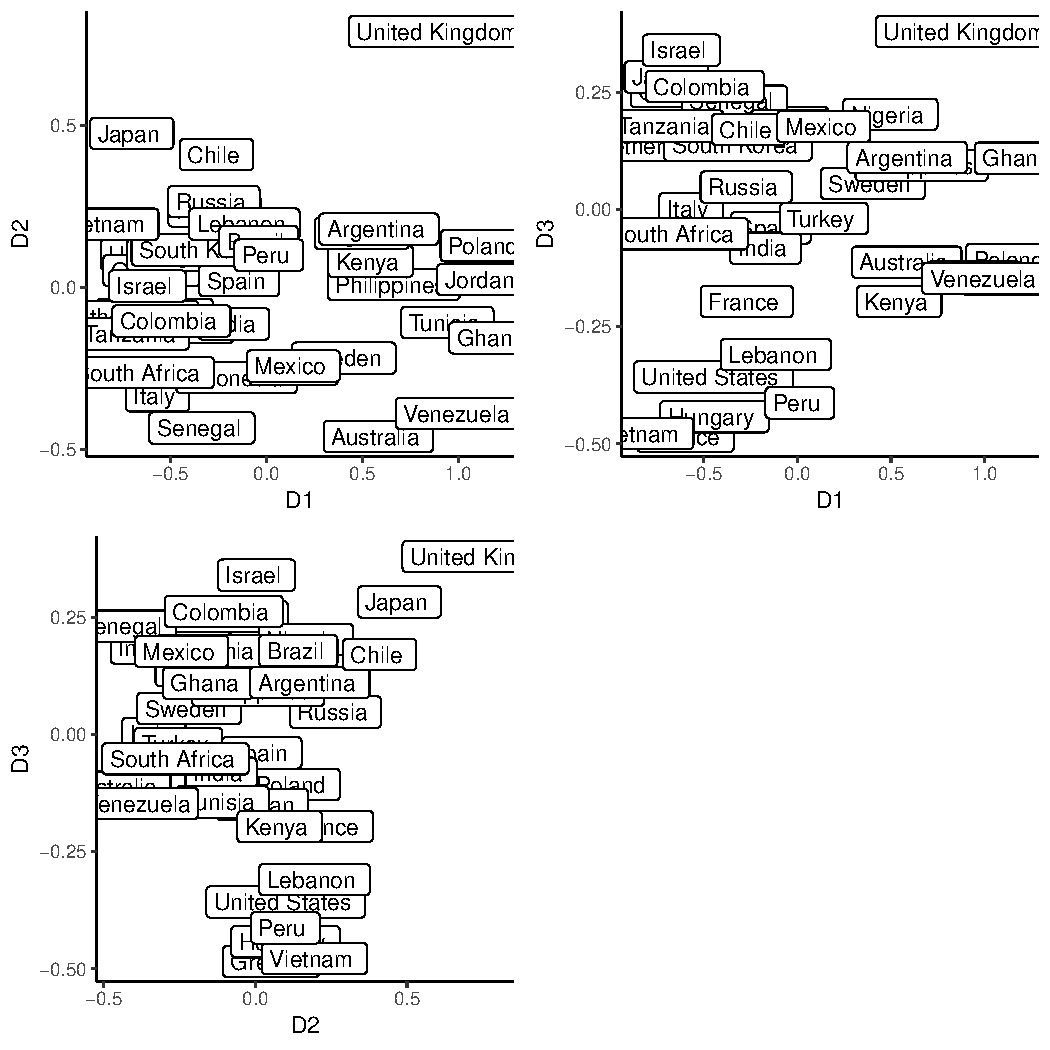
\includegraphics[width=\maxwidth]{figure/unnamed-chunk-11-1} 

\end{knitrout}

\section{Question 7}
Examine the multidimensional space and provide names for the dimensions.  
\begin{knitrout}
\definecolor{shadecolor}{rgb}{0.969, 0.969, 0.969}\color{fgcolor}\begin{kframe}
\begin{alltt}
\hlstd{mds_3_dat} \hlkwb{<-} \hlstd{mds_3_dat} \hlopt
  \hlkwd{mutate}\hlstd{(}\hlkwc{Country} \hlstd{=} \hlkwd{str_remove_all}\hlstd{(}\hlkwd{unique}\hlstd{(dat}\hlopt{$}\hlstd{Country),} \hlstr{" "}\hlstd{))}

\hlstd{p1} \hlkwb{<-} \hlstd{mds_3_dat} \hlopt
  \hlkwd{ggplot}\hlstd{(}\hlkwd{aes}\hlstd{(}\hlkwc{x} \hlstd{= D1,} \hlkwc{y} \hlstd{= D2,} \hlkwc{label} \hlstd{= Country))} \hlopt{+}
    \hlkwd{geom_text}\hlstd{()} \hlopt{+}
    \hlkwd{theme_classic}\hlstd{()}

\hlstd{p2} \hlkwb{<-} \hlstd{mds_3_dat} \hlopt
  \hlkwd{ggplot}\hlstd{(}\hlkwd{aes}\hlstd{(}\hlkwc{x} \hlstd{= D1,} \hlkwc{y} \hlstd{= D3,} \hlkwc{label} \hlstd{= Country))} \hlopt{+}
    \hlkwd{geom_text}\hlstd{()} \hlopt{+}
    \hlkwd{theme_classic}\hlstd{()}

\hlstd{p3} \hlkwb{<-} \hlstd{mds_3_dat} \hlopt
  \hlkwd{ggplot}\hlstd{(}\hlkwd{aes}\hlstd{(}\hlkwc{x} \hlstd{= D2,} \hlkwc{y} \hlstd{= D3,} \hlkwc{label} \hlstd{= Country))} \hlopt{+}
    \hlkwd{geom_text}\hlstd{()} \hlopt{+}
    \hlkwd{theme_classic}\hlstd{()}

\hlstd{gridExtra}\hlopt{::}\hlkwd{grid.arrange}\hlstd{(p1, p2, p3,} \hlkwc{nrow} \hlstd{=} \hlnum{1}\hlstd{)}
\end{alltt}
\end{kframe}
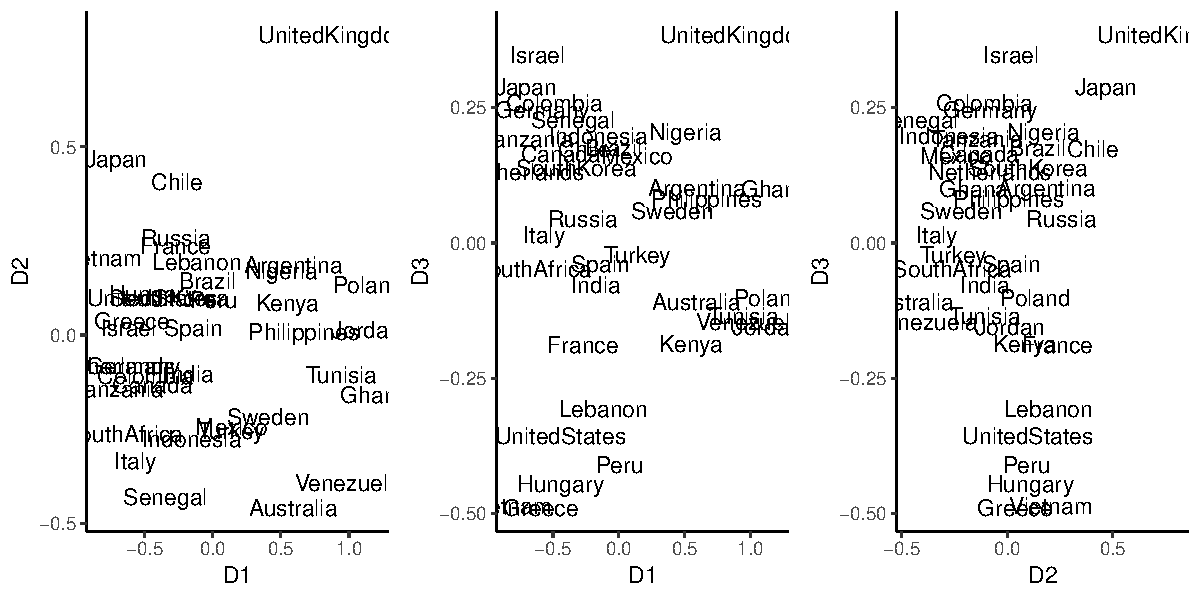
\includegraphics[width=\maxwidth]{figure/unnamed-chunk-12-1} 

\end{knitrout}

Dimension 1 might be general support for Trump. Dimension 2 might be egalitarianism. Dimension 3 could be Liberalism.

\section{Question 8}
Are there any clusters of countries that seem to emerge in the multidimensional space? Provide the same profile plot for each cluster as you provided for all countries in Question 1.
Columbia, Germany, the Netherlands, Indonesia, Brazil, South Korea, Canada, and Tanzania seem to cluster together across all 3 dimensions.

\begin{knitrout}
\definecolor{shadecolor}{rgb}{0.969, 0.969, 0.969}\color{fgcolor}\begin{kframe}
\begin{alltt}
\hlstd{dat} \hlopt
  \hlkwd{mutate}\hlstd{(}\hlkwc{Country} \hlstd{=} \hlkwd{str_remove_all}\hlstd{(Country,} \hlstr{" "}\hlstd{),}
         \hlkwc{cluster} \hlstd{=} \hlkwd{ifelse}\hlstd{(Country} \hlopt \hlkwd{c}\hlstd{(}\hlstr{"Colombia"}\hlstd{,} \hlstr{"Germany"}\hlstd{,} \hlstr{"Netherlands"}\hlstd{,}
         \hlstr{"Indonesia"}\hlstd{,} \hlstr{"Brazil"}\hlstd{,} \hlstr{"South Korea"}\hlstd{,} \hlstr{"Canada"}\hlstd{,} \hlstr{"Tanzania"}\hlstd{),} \hlstr{"Cluster"}\hlstd{, Country))} \hlopt
  \hlkwd{gather}\hlstd{(}\hlkwc{key} \hlstd{= item,} \hlkwc{value} \hlstd{= value,} \hlopt{-}\hlstd{Country,} \hlopt{-}\hlstd{cluster)} \hlopt
  \hlstd{Rmisc}\hlopt{::}\hlkwd{summarySE}\hlstd{(.,} \hlkwc{measurevar} \hlstd{=} \hlstr{"value"}\hlstd{,} \hlkwc{groupvars} \hlstd{=} \hlstr{"item"}\hlstd{)} \hlopt
  \hlkwd{mutate}\hlstd{(}\hlkwc{rank} \hlstd{=} \hlkwd{rank}\hlstd{(}\hlkwd{desc}\hlstd{(value)))} \hlopt
  \hlkwd{arrange}\hlstd{(rank)} \hlopt
  \hlkwd{mutate}\hlstd{(}\hlkwc{item} \hlstd{=} \hlkwd{factor}\hlstd{(item,} \hlkwc{levels} \hlstd{=} \hlkwd{unique}\hlstd{(item)))} \hlopt
  \hlkwd{ggplot}\hlstd{(}\hlkwd{aes}\hlstd{(}\hlkwc{x} \hlstd{= item,} \hlkwc{y} \hlstd{= value,} \hlkwc{ymin} \hlstd{= value} \hlopt{-} \hlstd{ci,} \hlkwc{ymax} \hlstd{= value} \hlopt{+} \hlstd{ci))} \hlopt{+}
    \hlkwd{geom_bar}\hlstd{(}\hlkwd{aes}\hlstd{(}\hlkwc{fill} \hlstd{= item),} \hlkwc{color} \hlstd{=} \hlstr{"black"}\hlstd{,} \hlkwc{position} \hlstd{=} \hlstr{"dodge"}\hlstd{,} \hlkwc{stat} \hlstd{=} \hlstr{"identity"}\hlstd{)} \hlopt{+}
    \hlkwd{geom_errorbar}\hlstd{(}\hlkwc{position} \hlstd{=} \hlstr{"dodge"}\hlstd{,} \hlkwc{width} \hlstd{=} \hlnum{.1}\hlstd{)} \hlopt{+}
    \hlkwd{labs}\hlstd{(}\hlkwc{y} \hlstd{=} \hlstr{"Mean Percentage"}\hlstd{,} \hlkwc{x} \hlstd{=} \hlkwa{NULL}\hlstd{)} \hlopt{+}
    \hlkwd{coord_flip}\hlstd{()} \hlopt{+}
    \hlkwd{theme_classic}\hlstd{()} \hlopt{+}
    \hlkwd{theme}\hlstd{(}\hlkwc{legend.position} \hlstd{=} \hlstr{"none"}\hlstd{)}
\end{alltt}
\end{kframe}
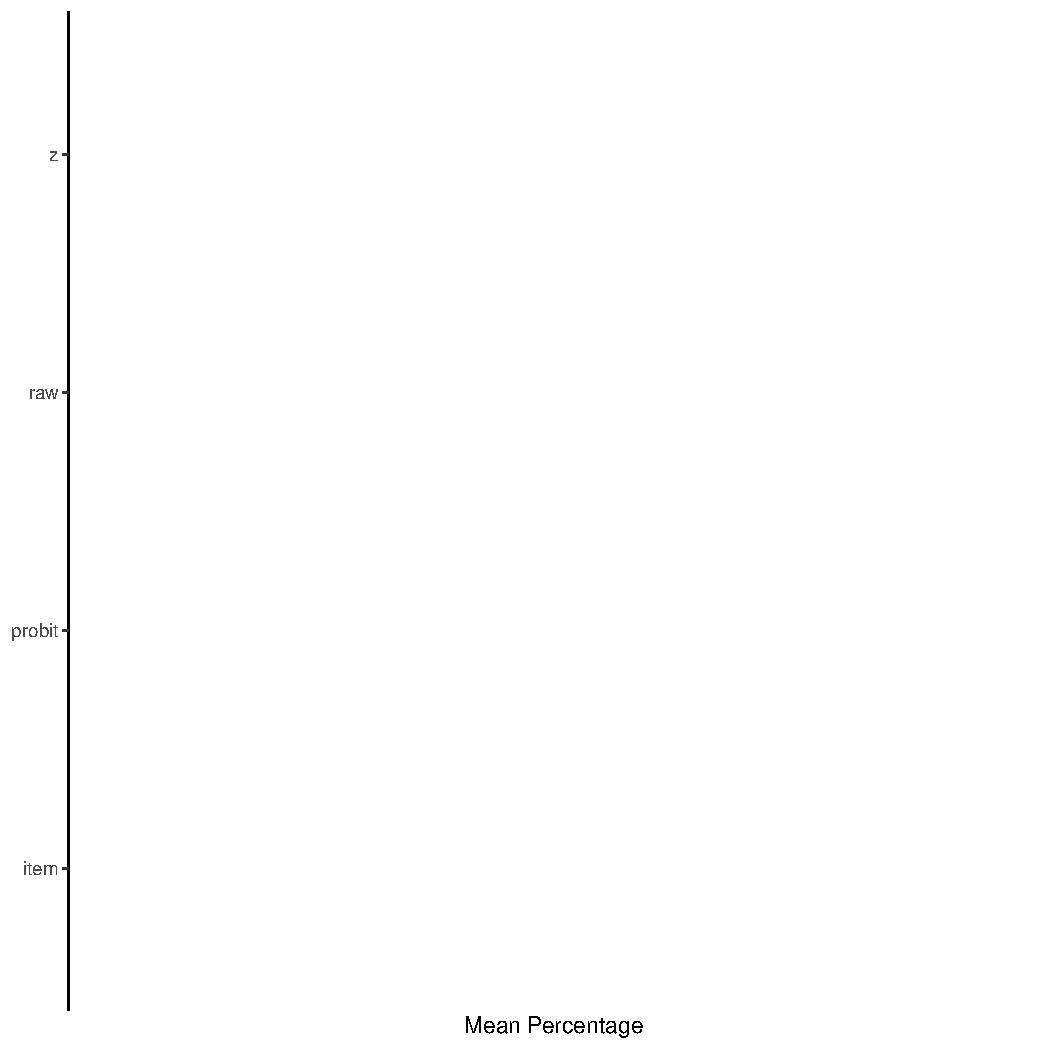
\includegraphics[width=\maxwidth]{figure/unnamed-chunk-13-1} 

\end{knitrout}



\section{Question 9}
Repeat the analyses using the standardized ratings. Comment on any differences that you observe.  
\begin{knitrout}
\definecolor{shadecolor}{rgb}{0.969, 0.969, 0.969}\color{fgcolor}\begin{kframe}
\begin{alltt}
\hlcom{# stress plot}
\hlstd{nested.dat} \hlopt
  \hlkwd{filter}\hlstd{(type} \hlopt{==} \hlstr{"z"}\hlstd{)} \hlopt
  \hlkwd{ggplot}\hlstd{(}\hlkwd{aes}\hlstd{(}\hlkwc{x} \hlstd{= dim,} \hlkwc{y} \hlstd{= stress))} \hlopt{+}
    \hlkwd{geom_line}\hlstd{()} \hlopt{+}
    \hlkwd{geom_point}\hlstd{()} \hlopt{+}
    \hlkwd{scale_x_continuous}\hlstd{(}\hlkwc{limits} \hlstd{=} \hlkwd{c}\hlstd{(}\hlnum{1}\hlstd{,}\hlnum{6}\hlstd{),} \hlkwc{breaks} \hlstd{=} \hlnum{1}\hlopt{:}\hlnum{6}\hlstd{)} \hlopt{+}
    \hlkwd{labs}\hlstd{(}\hlkwc{x} \hlstd{=} \hlstr{"Number of Dimensions"}\hlstd{,} \hlkwc{y} \hlstd{=} \hlstr{"Stress"}\hlstd{,} \hlkwc{title} \hlstd{=} \hlstr{"Question 9: Stress Plot"}\hlstd{)} \hlopt{+}
    \hlkwd{theme_classic}\hlstd{()} \hlopt{+}
    \hlkwd{theme}\hlstd{(}\hlkwc{plot.title} \hlstd{=} \hlkwd{element_text}\hlstd{(}\hlkwc{face} \hlstd{=} \hlstr{"bold"}\hlstd{,} \hlkwc{hjust} \hlstd{=} \hlnum{.5}\hlstd{),}
          \hlkwc{axis.text} \hlstd{=} \hlkwd{element_text}\hlstd{(}\hlkwc{face} \hlstd{=} \hlstr{"bold"}\hlstd{,} \hlkwc{color} \hlstd{=} \hlstr{"black"}\hlstd{),}
          \hlkwc{axis.title} \hlstd{=} \hlkwd{element_text}\hlstd{(}\hlkwc{face} \hlstd{=} \hlstr{"bold"}\hlstd{))}
\end{alltt}
\end{kframe}
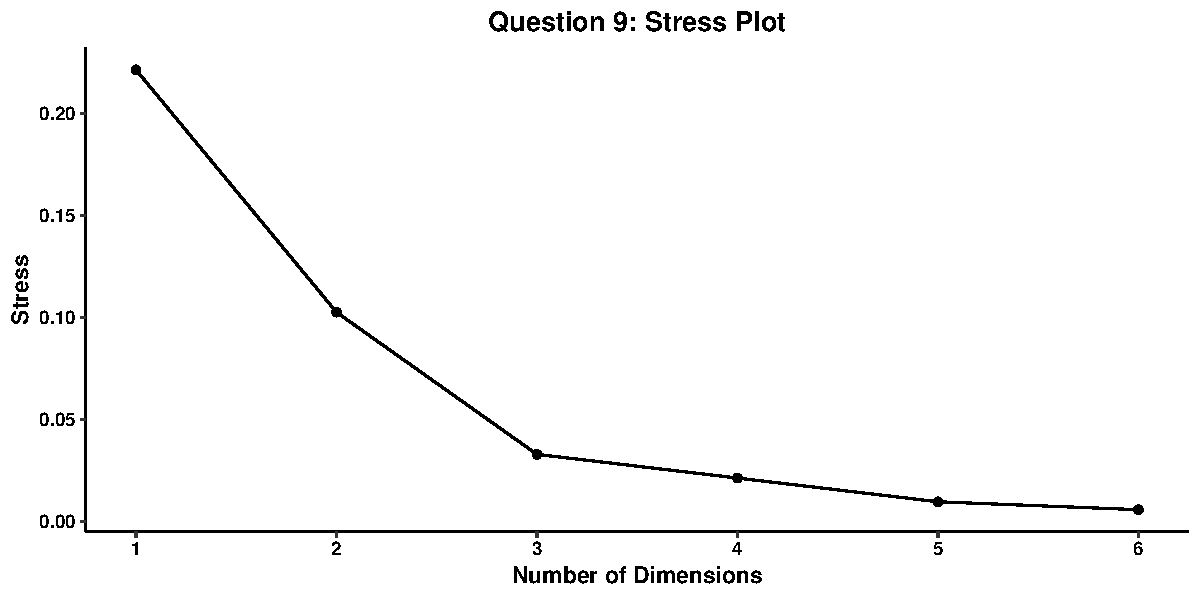
\includegraphics[width=\maxwidth]{figure/unnamed-chunk-14-1} 
\begin{kframe}\begin{alltt}
\hlcom{# shepard plot}
\hlstd{nested.dat} \hlopt
  \hlkwd{unnest}\hlstd{(shep_val)} \hlopt
  \hlkwd{filter}\hlstd{(dim} \hlopt{<=} \hlnum{4} \hlopt{&} \hlstd{type} \hlopt{==} \hlstr{"z"}\hlstd{)} \hlopt
  \hlkwd{ggplot}\hlstd{(}\hlkwd{aes}\hlstd{(}\hlkwc{x} \hlstd{= Dissimilarity,} \hlkwc{y} \hlstd{= Distance,} \hlkwc{color} \hlstd{=} \hlkwd{factor}\hlstd{(dim)))} \hlopt{+}
    \hlkwd{geom_point}\hlstd{()} \hlopt{+}
    \hlkwd{facet_wrap}\hlstd{(}\hlopt{~}\hlstd{dim)} \hlopt{+}
    \hlkwd{theme_classic}\hlstd{()} \hlopt{+}
    \hlkwd{theme}\hlstd{(}\hlkwc{legend.position} \hlstd{=} \hlstr{"none"}\hlstd{)}
\end{alltt}
\end{kframe}
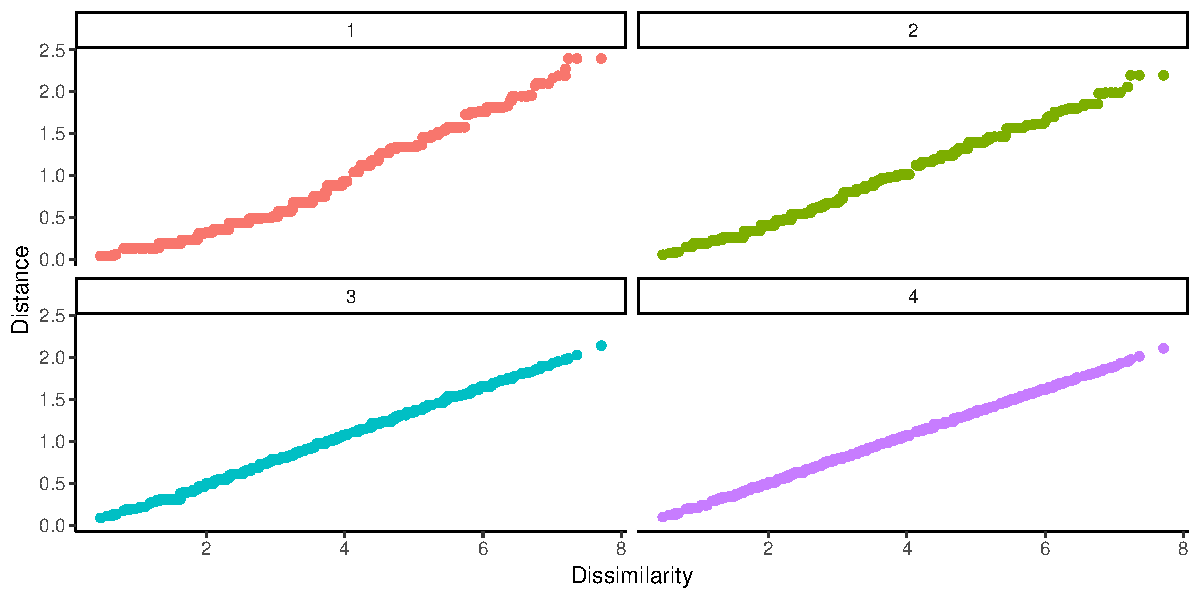
\includegraphics[width=\maxwidth]{figure/unnamed-chunk-14-2} 
\begin{kframe}\begin{alltt}
\hlcom{# mds}
\hlstd{mds_3_dat_z} \hlkwb{<-} \hlstd{(nested.dat} \hlopt
  \hlkwd{filter}\hlstd{(dim} \hlopt{==} \hlnum{3} \hlopt{&} \hlstd{type} \hlopt{==} \hlstr{"z"}\hlstd{))}\hlopt{$}\hlstd{mds[[}\hlnum{1}\hlstd{]]}\hlopt{$}\hlstd{conf} \hlopt
  \hlstd{data.frame}

\hlkwd{scatterplot3d}\hlstd{(}\hlkwc{x} \hlstd{= mds_3_dat_z}\hlopt{$}\hlstd{D1,} \hlkwc{y} \hlstd{= mds_3_dat_z}\hlopt{$}\hlstd{D2,} \hlkwc{z} \hlstd{= mds_3_dat_z}\hlopt{$}\hlstd{D3,}
              \hlkwc{xlab} \hlstd{=} \hlstr{"Dimension 1"}\hlstd{,} \hlkwc{ylab} \hlstd{=} \hlstr{"Dimension 2"}\hlstd{,} \hlkwc{zlab} \hlstd{=} \hlstr{"Dimension 3x"}\hlstd{)}
\end{alltt}
\end{kframe}
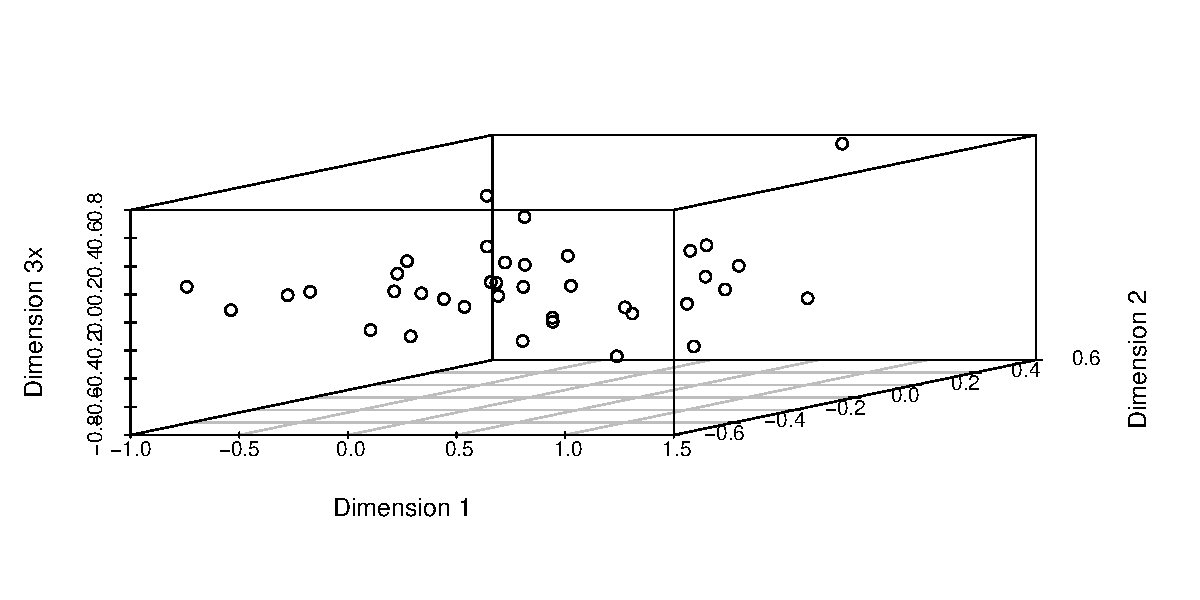
\includegraphics[width=\maxwidth]{figure/unnamed-chunk-14-3} 
\begin{kframe}\begin{alltt}
\hlstd{mds_3_dat_z} \hlkwb{<-} \hlstd{mds_3_dat_z} \hlopt
  \hlkwd{mutate}\hlstd{(}\hlkwc{Country} \hlstd{=} \hlkwd{str_remove_all}\hlstd{(}\hlkwd{unique}\hlstd{(dat}\hlopt{$}\hlstd{Country),} \hlstr{" "}\hlstd{))}

\hlstd{p1} \hlkwb{<-} \hlstd{mds_3_dat_z} \hlopt
  \hlkwd{ggplot}\hlstd{(}\hlkwd{aes}\hlstd{(}\hlkwc{x} \hlstd{= D1,} \hlkwc{y} \hlstd{= D2,} \hlkwc{label} \hlstd{= Country))} \hlopt{+}
    \hlkwd{geom_text}\hlstd{()} \hlopt{+}
    \hlkwd{theme_classic}\hlstd{()}

\hlstd{p2} \hlkwb{<-} \hlstd{mds_3_dat_z} \hlopt
  \hlkwd{ggplot}\hlstd{(}\hlkwd{aes}\hlstd{(}\hlkwc{x} \hlstd{= D1,} \hlkwc{y} \hlstd{= D3,} \hlkwc{label} \hlstd{= Country))} \hlopt{+}
    \hlkwd{geom_text}\hlstd{()} \hlopt{+}
    \hlkwd{theme_classic}\hlstd{()}

\hlstd{p3} \hlkwb{<-} \hlstd{mds_3_dat_z} \hlopt
  \hlkwd{ggplot}\hlstd{(}\hlkwd{aes}\hlstd{(}\hlkwc{x} \hlstd{= D2,} \hlkwc{y} \hlstd{= D3,} \hlkwc{label} \hlstd{= Country))} \hlopt{+}
    \hlkwd{geom_text}\hlstd{()} \hlopt{+}
    \hlkwd{theme_classic}\hlstd{()}

\hlstd{gridExtra}\hlopt{::}\hlkwd{grid.arrange}\hlstd{(p1, p2, p3,} \hlkwc{nrow} \hlstd{=} \hlnum{1}\hlstd{)}
\end{alltt}
\end{kframe}
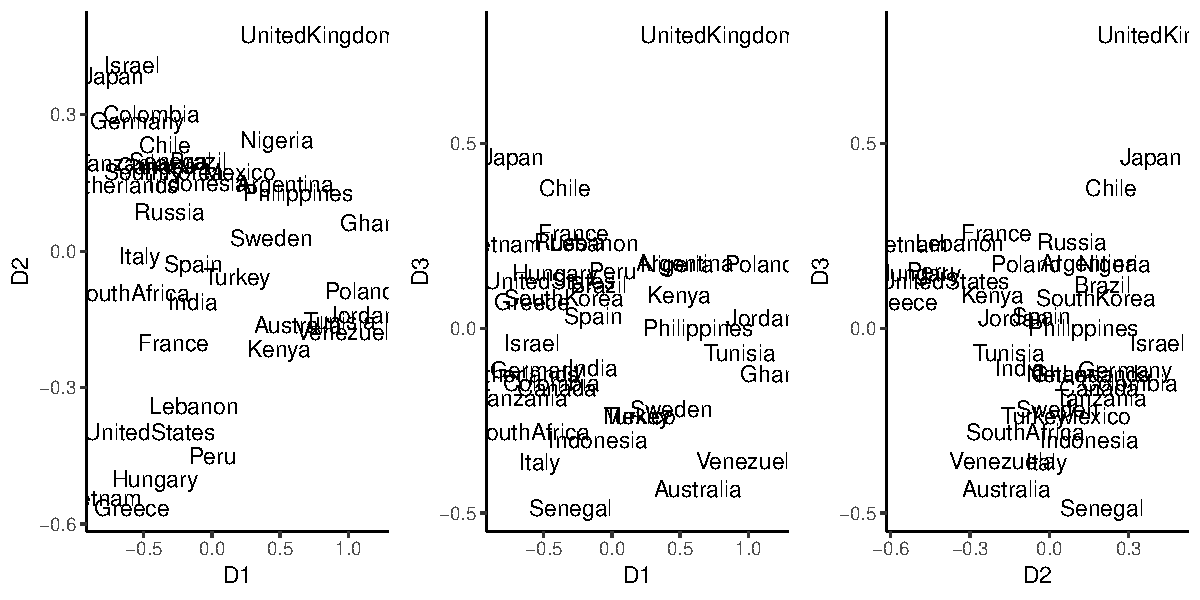
\includegraphics[width=\maxwidth]{figure/unnamed-chunk-14-4} 

\end{knitrout}

Nothing appears to change when using standardized scores, so the dimension names, etc. would be the same.

\section{Question 10}
Repeat the analyses using the probits. Comment on any differences that you observe.
\begin{knitrout}
\definecolor{shadecolor}{rgb}{0.969, 0.969, 0.969}\color{fgcolor}\begin{kframe}
\begin{alltt}
\hlcom{# stress plot}
\hlstd{nested.dat} \hlopt
  \hlkwd{filter}\hlstd{(type} \hlopt{==} \hlstr{"probit"}\hlstd{)} \hlopt
  \hlkwd{ggplot}\hlstd{(}\hlkwd{aes}\hlstd{(}\hlkwc{x} \hlstd{= dim,} \hlkwc{y} \hlstd{= stress))} \hlopt{+}
    \hlkwd{geom_line}\hlstd{()} \hlopt{+}
    \hlkwd{geom_point}\hlstd{()} \hlopt{+}
    \hlkwd{scale_x_continuous}\hlstd{(}\hlkwc{limits} \hlstd{=} \hlkwd{c}\hlstd{(}\hlnum{1}\hlstd{,}\hlnum{6}\hlstd{),} \hlkwc{breaks} \hlstd{=} \hlnum{1}\hlopt{:}\hlnum{6}\hlstd{)} \hlopt{+}
    \hlkwd{labs}\hlstd{(}\hlkwc{x} \hlstd{=} \hlstr{"Number of Dimensions"}\hlstd{,} \hlkwc{y} \hlstd{=} \hlstr{"Stress"}\hlstd{,} \hlkwc{title} \hlstd{=} \hlstr{"Question 9: Stress Plot"}\hlstd{)} \hlopt{+}
    \hlkwd{theme_classic}\hlstd{()} \hlopt{+}
    \hlkwd{theme}\hlstd{(}\hlkwc{plot.title} \hlstd{=} \hlkwd{element_text}\hlstd{(}\hlkwc{face} \hlstd{=} \hlstr{"bold"}\hlstd{,} \hlkwc{hjust} \hlstd{=} \hlnum{.5}\hlstd{),}
          \hlkwc{axis.text} \hlstd{=} \hlkwd{element_text}\hlstd{(}\hlkwc{face} \hlstd{=} \hlstr{"bold"}\hlstd{,} \hlkwc{color} \hlstd{=} \hlstr{"black"}\hlstd{),}
          \hlkwc{axis.title} \hlstd{=} \hlkwd{element_text}\hlstd{(}\hlkwc{face} \hlstd{=} \hlstr{"bold"}\hlstd{))}
\end{alltt}
\end{kframe}
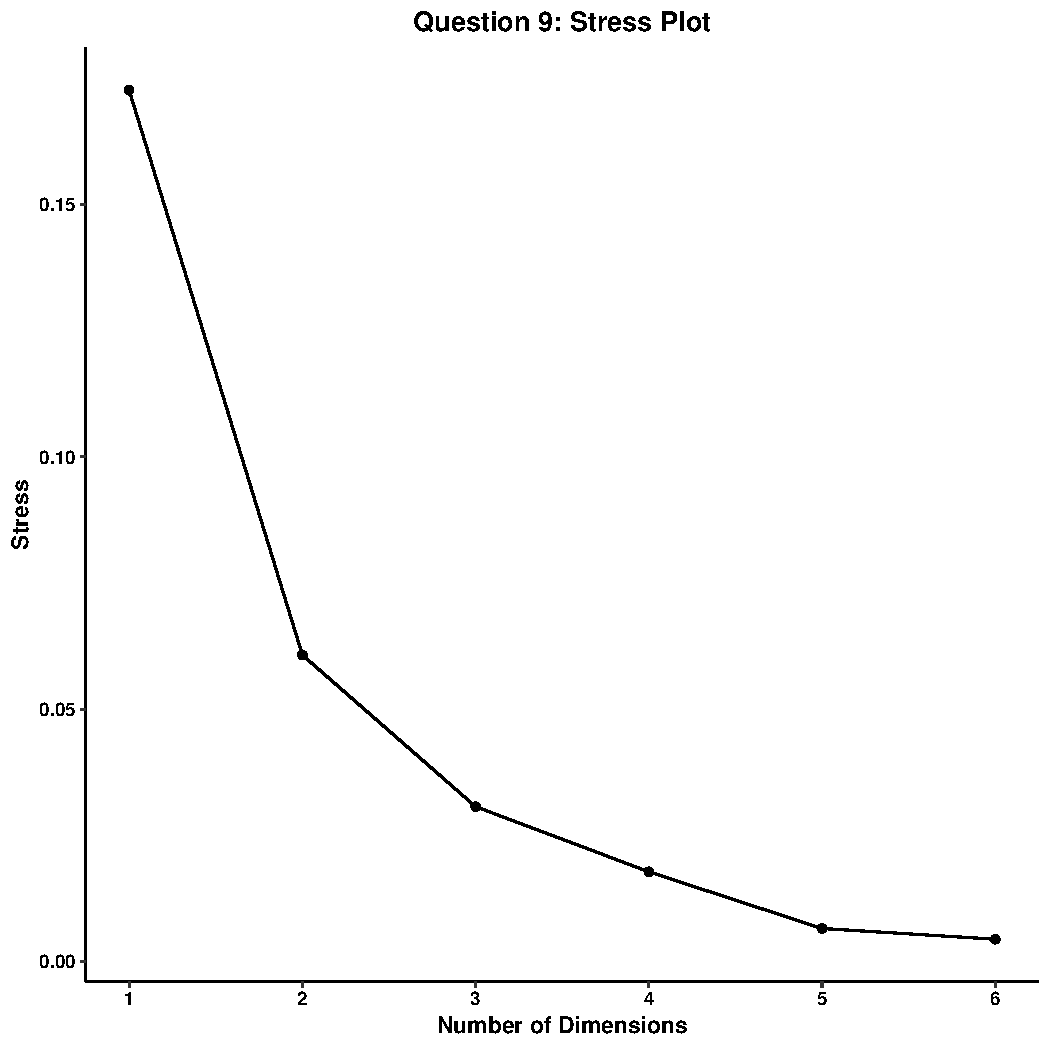
\includegraphics[width=\maxwidth]{figure/unnamed-chunk-15-1} 
\begin{kframe}\begin{alltt}
\hlcom{# shepard plot}
\hlstd{nested.dat} \hlopt
  \hlkwd{unnest}\hlstd{(shep_val)} \hlopt
  \hlkwd{filter}\hlstd{(dim} \hlopt{<=} \hlnum{6} \hlopt{&} \hlstd{type} \hlopt{==} \hlstr{"probit"}\hlstd{)} \hlopt
  \hlkwd{ggplot}\hlstd{(}\hlkwd{aes}\hlstd{(}\hlkwc{x} \hlstd{= Dissimilarity,} \hlkwc{y} \hlstd{= Distance,} \hlkwc{color} \hlstd{=} \hlkwd{factor}\hlstd{(dim)))} \hlopt{+}
    \hlkwd{geom_point}\hlstd{()} \hlopt{+}
    \hlkwd{facet_wrap}\hlstd{(}\hlopt{~}\hlstd{dim)} \hlopt{+}
    \hlkwd{theme_classic}\hlstd{()} \hlopt{+}
    \hlkwd{theme}\hlstd{(}\hlkwc{legend.position} \hlstd{=} \hlstr{"none"}\hlstd{)}
\end{alltt}
\end{kframe}
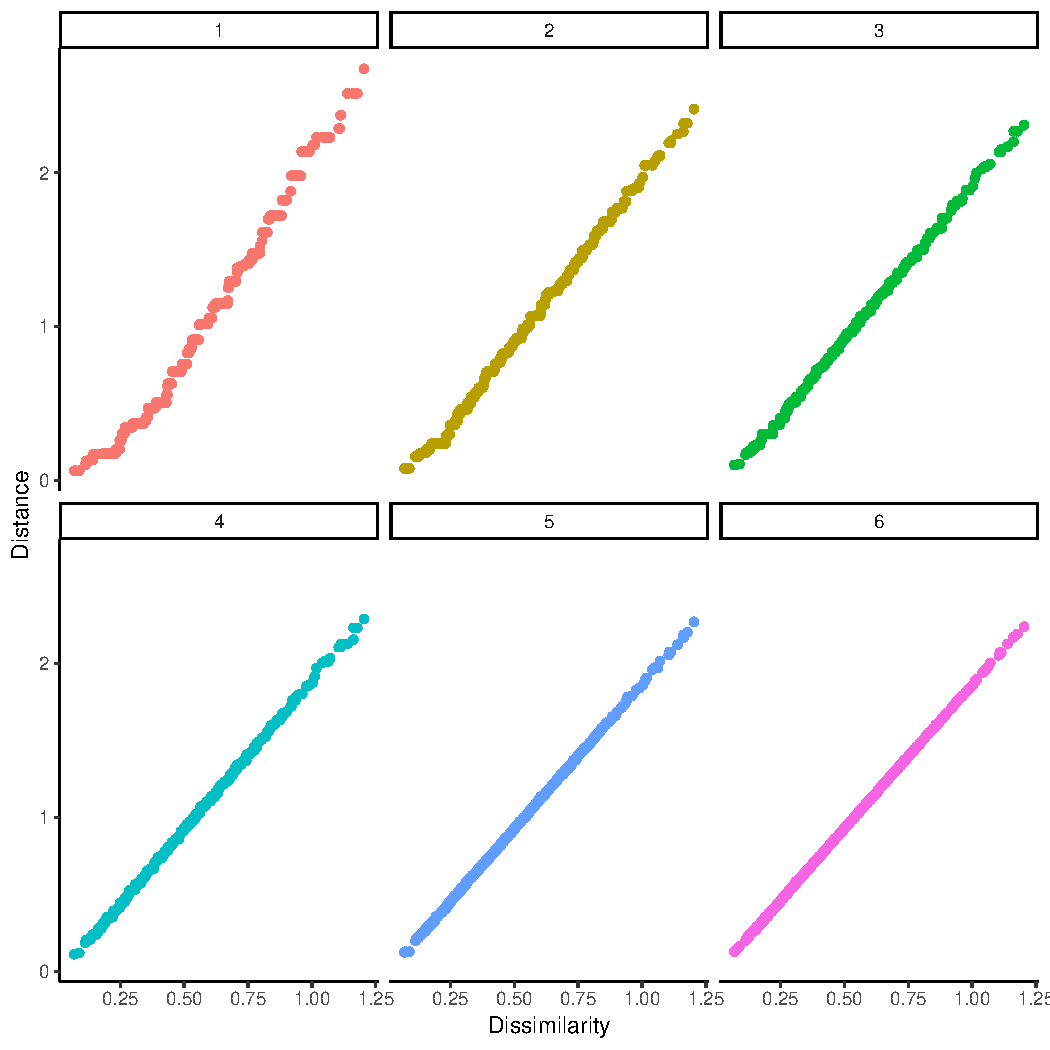
\includegraphics[width=\maxwidth]{figure/unnamed-chunk-15-2} 

\end{knitrout}

\begin{knitrout}
\definecolor{shadecolor}{rgb}{0.969, 0.969, 0.969}\color{fgcolor}\begin{kframe}
\begin{alltt}
\hlcom{# mds}
\hlstd{mds_3_dat_p} \hlkwb{<-} \hlstd{(nested.dat} \hlopt
  \hlkwd{filter}\hlstd{(dim} \hlopt{==} \hlnum{4} \hlopt{&} \hlstd{type} \hlopt{==} \hlstr{"probit"}\hlstd{))}\hlopt{$}\hlstd{mds[[}\hlnum{1}\hlstd{]]}\hlopt{$}\hlstd{conf} \hlopt
  \hlstd{data.frame}

\hlstd{mds_3_dat_p} \hlkwb{<-} \hlstd{mds_3_dat_p} \hlopt
  \hlkwd{mutate}\hlstd{(}\hlkwc{Country} \hlstd{=} \hlkwd{str_remove_all}\hlstd{(}\hlkwd{unique}\hlstd{(dat}\hlopt{$}\hlstd{Country),} \hlstr{" "}\hlstd{))}

\hlstd{p1} \hlkwb{<-} \hlstd{mds_3_dat_p} \hlopt
  \hlkwd{ggplot}\hlstd{(}\hlkwd{aes}\hlstd{(}\hlkwc{x} \hlstd{= D1,} \hlkwc{y} \hlstd{= D2,} \hlkwc{label} \hlstd{= Country))} \hlopt{+}
    \hlkwd{geom_text}\hlstd{()} \hlopt{+}
    \hlkwd{theme_classic}\hlstd{()}

\hlstd{p2} \hlkwb{<-} \hlstd{mds_3_dat_p} \hlopt
  \hlkwd{ggplot}\hlstd{(}\hlkwd{aes}\hlstd{(}\hlkwc{x} \hlstd{= D1,} \hlkwc{y} \hlstd{= D3,} \hlkwc{label} \hlstd{= Country))} \hlopt{+}
    \hlkwd{geom_text}\hlstd{()} \hlopt{+}
    \hlkwd{theme_classic}\hlstd{()}

\hlstd{p3} \hlkwb{<-} \hlstd{mds_3_dat_p} \hlopt
  \hlkwd{ggplot}\hlstd{(}\hlkwd{aes}\hlstd{(}\hlkwc{x} \hlstd{= D1,} \hlkwc{y} \hlstd{= D4,} \hlkwc{label} \hlstd{= Country))} \hlopt{+}
    \hlkwd{geom_text}\hlstd{()} \hlopt{+}
    \hlkwd{theme_classic}\hlstd{()}

\hlstd{p4} \hlkwb{<-} \hlstd{mds_3_dat_p} \hlopt
  \hlkwd{ggplot}\hlstd{(}\hlkwd{aes}\hlstd{(}\hlkwc{x} \hlstd{= D2,} \hlkwc{y} \hlstd{= D3,} \hlkwc{label} \hlstd{= Country))} \hlopt{+}
    \hlkwd{geom_text}\hlstd{()} \hlopt{+}
    \hlkwd{theme_classic}\hlstd{()}

\hlstd{p5} \hlkwb{<-} \hlstd{mds_3_dat_p} \hlopt
  \hlkwd{ggplot}\hlstd{(}\hlkwd{aes}\hlstd{(}\hlkwc{x} \hlstd{= D2,} \hlkwc{y} \hlstd{= D4,} \hlkwc{label} \hlstd{= Country))} \hlopt{+}
    \hlkwd{geom_text}\hlstd{()} \hlopt{+}
    \hlkwd{theme_classic}\hlstd{()}

\hlstd{p6} \hlkwb{<-} \hlstd{mds_3_dat_p} \hlopt
  \hlkwd{ggplot}\hlstd{(}\hlkwd{aes}\hlstd{(}\hlkwc{x} \hlstd{= D3,} \hlkwc{y} \hlstd{= D4,} \hlkwc{label} \hlstd{= Country))} \hlopt{+}
    \hlkwd{geom_text}\hlstd{()} \hlopt{+}
    \hlkwd{theme_classic}\hlstd{()}

\hlstd{gridExtra}\hlopt{::}\hlkwd{grid.arrange}\hlstd{(p1, p2, p3, p4, p5, p6,} \hlkwc{nrow} \hlstd{=} \hlnum{2}\hlstd{)}
\end{alltt}
\end{kframe}
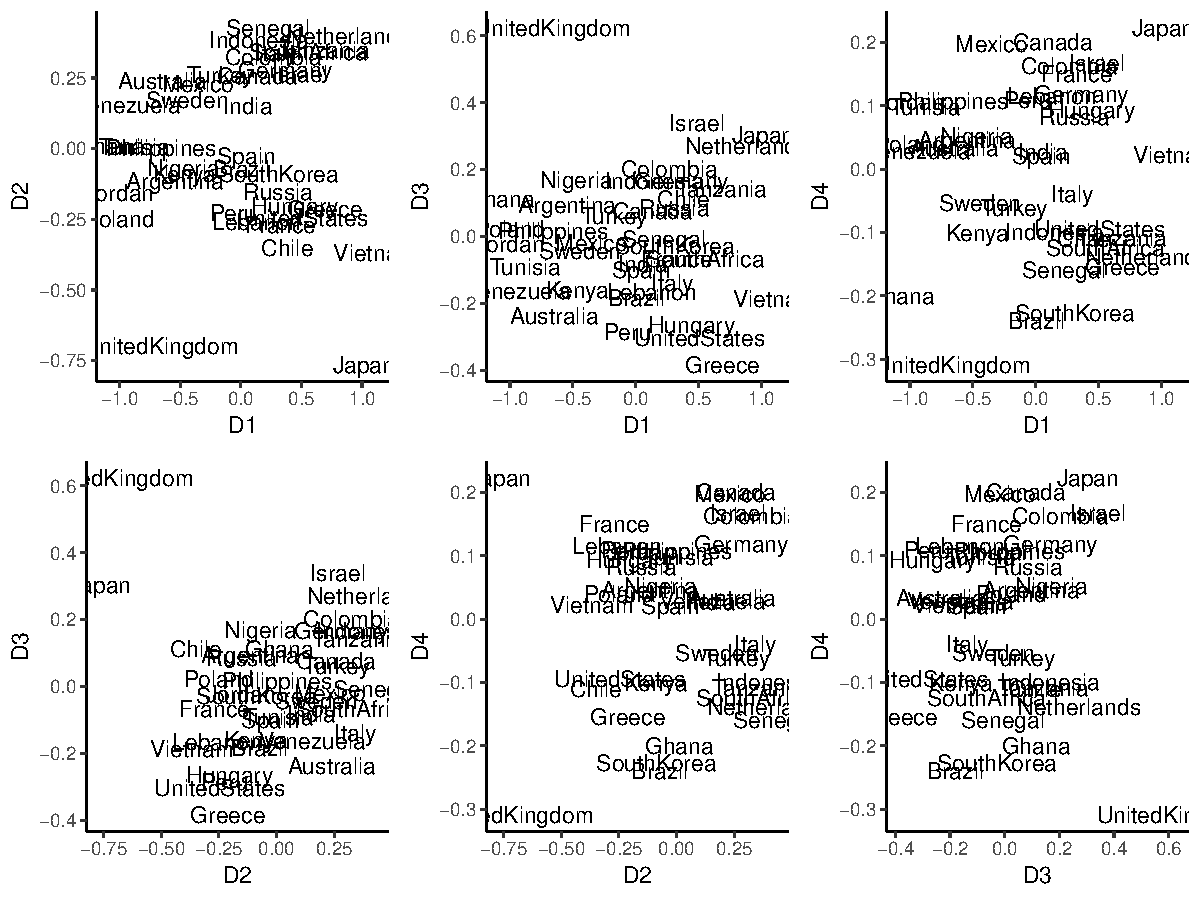
\includegraphics[width=\maxwidth]{figure/unnamed-chunk-16-1} 

\end{knitrout}
Using Probit, 4 dimensions appears to be the best solution, both per the Shepard and stress plots. In this soltuion, the UK is finally low on something (Dimensions 1 and 4), suggesting that the fundamental nature of the dimensions has changed. Moreover, on Dimension 4, the countries that clustered together when using raw scores do not seem to cluster together on this dimension.  


\end{document}
